\documentclass[13pt,onlymath]{beamer}
\usefonttheme{serif}
\usepackage{graphicx,amsmath,amssymb,tikz,psfrag,epstopdf,fancyvrb}
\usepackage[lighttt]{lmodern}
%\usepackage{graphicx,psfrag}

\input defs.tex

%% formatting

\mode<presentation>
{
\usetheme{default}
}
\setbeamertemplate{navigation symbols}{}
\usecolortheme[rgb={0.13,0.28,0.59}]{structure}
\setbeamertemplate{itemize subitem}{--}
\setbeamertemplate{frametitle} {
    \begin{center}
      {\large\bf \insertframetitle}
    \end{center}
}

\newcommand\footlineon{
  \setbeamertemplate{footline} {
    \begin{beamercolorbox}[ht=2.5ex,dp=1.125ex,leftskip=.8cm,rightskip=.6cm]{structure}
      \footnotesize \insertsection
      \hfill
      {\insertframenumber}
    \end{beamercolorbox}
    \vskip 0.45cm
  }
}
\footlineon

\AtBeginSection[] 
{ 
    \begin{frame}<beamer> 
        \frametitle{Outline} 
        \tableofcontents[currentsection,currentsubsection] 
    \end{frame} 
} 

%% begin presentation

\title{\large \bfseries Data Structures}

\author{Jaehyun Park\\[3ex]
CS 97SI\\
Stanford University}

\date{\today}

\begin{document}

\frame{
\thispagestyle{empty}
\titlepage
}

\begin{frame}[fragile]{Typical Quarter at Stanford}
\begin{Verbatim}[xleftmargin=25pt]
void quarter() {
    while(true) { // no break :(
        task x = GetNextTask(tasks);
        process(x);
        // new tasks may enter
    }
}
\end{Verbatim}
\BIT
\item \verb,GetNextTask(), decides the order of the tasks
\EIT
\end{frame}

\begin{frame}[fragile]{Deciding the Order of the Tasks}
\BIT
\item Possible behaviors of GetNextTask():
\BIT
\item Returns the newest task (stack)
\item Returns the oldest task (queue)
\item Returns the most urgent task (priority queue)
\item Returns the easiest task (priority queue)
\EIT
\vfill
\item \verb,GetNextTask(), should run fast
\BIT
\item We do this by storing the tasks in a clever way
\EIT
\EIT
\end{frame}

\section{Stack and Queue}

\begin{frame}[fragile]{Stack}
\BIT
\item Last in, first out (LIFO)
\item Supports three constant-time operations
\BIT
\item \verb,Push(x),: inserts \verb,x, into the stack
\item \verb,Pop(),: removes the newest item
\item \verb,Top(),: returns the newest item
\EIT
\vfill
\item Very easy to implement using an array
\EIT
\end{frame}

\begin{frame}[fragile]{Stack Implementation}
\BIT
\item Have a large enough array \verb,s[], and a counter \verb,k,, which starts at zero
\BIT
\item \verb,Push(x),: set \verb,s[k] = x, and increment \verb,k, by 1
\item \verb,Pop(),: decrement \verb,k, by 1
\item \verb,Top(),: returns \verb,s[k - 1], (error if \verb,k, is zero)
\EIT
\item C++ and Java have implementations of stack
\BIT
\item \verb,stack, (C++), \verb,Stack, (Java)
\EIT
\item But you should be able to implement it from scratch
\EIT
\end{frame}

\begin{frame}[fragile]{Queue}
\BIT
\item First in, first out (FIFO)
\item Supports three constant-time operations
\BIT
\item \verb,Enqueue(x),: inserts \verb,x, into the queue
\item \verb,Dequeue(),: removes the oldest item
\item \verb,Front(),: returns the oldest item
\EIT
\vfill
\item Implementation is similar to that of stack
\EIT
\end{frame}

\begin{frame}[fragile]{Queue Implementation}
\BIT
\item Assume that you know the total number of elements that enter the queue
\BIT
\item ... which allows you to use an array for implementation
\EIT
\item Maintain two indices \verb,head, and \verb,tail,
\BIT
\item \verb,Dequeue(), increments \verb,head,
\item \verb,Enqueue(), increments \verb,tail,
\item Use the value of \verb,tail - head, to check emptiness
\EIT
\item You can use \verb,queue, (C++) and \verb,Queue, (Java)
\EIT
\end{frame}


\section{Heap and Priority Queue}

\begin{frame}[fragile]{Priority Queue}
\BIT
\item Each element in a PQ has a priority value
\item Three operations:
\BIT
\item \verb.Insert(x, p).: inserts \verb,x, into the PQ, whose priority is \verb,p,
\item \verb,RemoveTop(),: removes the element with the highest priority
\item \verb,Top(),: returns the element with the highest priority
\EIT
\item All operations can be done quickly if implemented using a heap
\item \verb,priority_queue, (C++), \verb,PriorityQueue, (Java)
\EIT
\end{frame}

\begin{frame}[fragile]{Heap}
\BIT
\item Complete binary tree with the heap property:
\BIT
\item The value of a node $\ge$ values of its children
\EIT
\item The root node has the maximum value
\BIT
\item Constant-time \verb,top(), operation
\EIT
\item Inserting/removing a node can be done in $O(\log n)$ time without breaking the heap property
\BIT
\item May need rearrangement of some nodes
\EIT
\EIT
\end{frame}

\begin{frame}{Heap Example}
\begin{center}
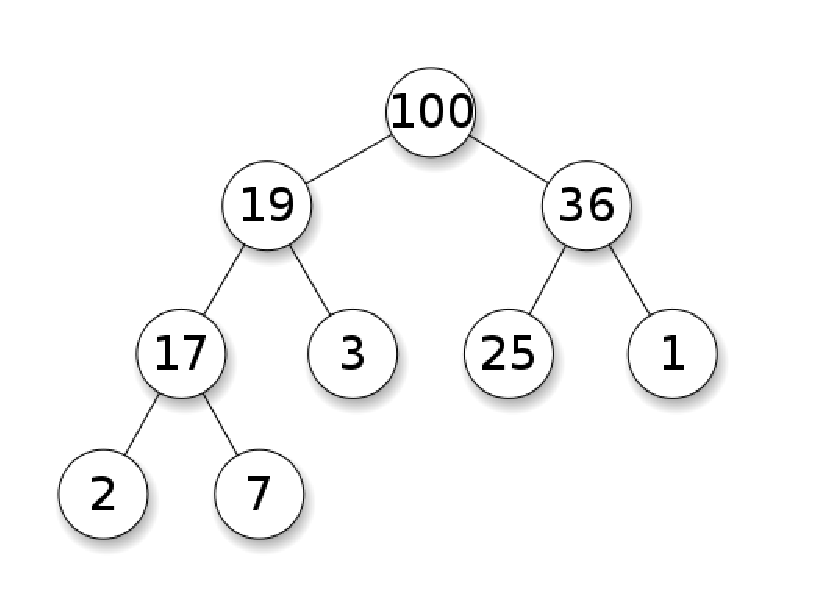
\includegraphics[height=0.5\textheight]{figures/heap}

Figure from Wikipedia
\end{center}
\end{frame}

\begin{frame}{Indexing the Nodes}
\begin{center}
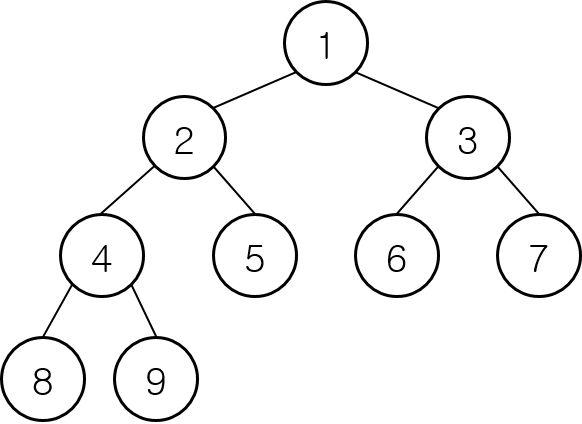
\includegraphics[height=0.4\textheight]{figures/heap_index}
\end{center}
\BIT
\item Start from the root, number the nodes $1, 2, \ldots$ from left to right
\item Given a node $k$ easy to compute the indices of its parent and children
\BIT
\item Parent node: $\lfloor k/2 \rfloor$
\item Children: $2k, 2k+1$
\EIT
\EIT
\end{frame}

\begin{frame}{Inserting a Node}
\begin{enumerate}
\item Make a new node in the last level, as far left as possible
\BIT
\item If the last level is full, make a new one
\EIT
\item If the new node breaks the heap property, swap with its parent node
\BIT
\item The new node moves up the tree, which may introduce another conflict
\EIT
\item Repeat 2 until all conflicts are resolved
\end{enumerate}
\BIT
\item Running time $=$ tree height $= O(\log n)$
\EIT
\end{frame}

\begin{frame}[fragile]{Implementation: Node Insertion}
\BIT
\item Inserting a new node with value v into a heap H
\EIT
\begin{Verbatim}[xleftmargin=25pt]
void InsertNode(int v) {
    H[++n] = v;
    for(int k = n; k > 1; k /= 2) {
        if(H[k] > H[k / 2])
            swap(H[k], H[k / 2]);
        else break;
    }
}
\end{Verbatim}
\end{frame}

\begin{frame}[fragile]{Deleting the Root Node}
\begin{enumerate}
\item Remove the root, and bring the last node (rightmost node in the last level) to the root
\item If the root breaks the heap property, look at its children and swap it with the larger one
\BIT
\item Swapping can introduce another conflict
\EIT
\item Repeat 2 until all conflicts are resolved
\end{enumerate}
\BIT
\item Running time $= O(\log n)$
\item Exercise: implementation
\BIT
\item Some edge cases to consider
\EIT
\EIT
\end{frame}


\section{Union-Find Structure}

\begin{frame}[fragile]{Union-Find Structure}
\BIT
\item Used to store disjoint sets
\item Can support two types of operations efficiently
\BIT
\item \verb,Find(x),: returns the ``representative'' of the set that \verb,x, belongs
\item \verb.Union(x, y).: merges two sets that contain \verb,x, and \verb,y,
\EIT
\vfill
\item Both operations can be done in (essentially) constant time
\item Super-short implementation!
\EIT
\end{frame}

\begin{frame}[fragile]{Union-Find Structure}
\BIT
\item Main idea: represent each set by a rooted tree
\BIT
\item Every node maintains a link to its parent
\item A root node is the ``representative'' of the corresponding set
\item Example: two sets $\{\mathtt{x}, \mathtt{y}, \mathtt{z}\}$ and $\{\mathtt{a}, \mathtt{b}, \mathtt{c}, \mathtt{d}\}$\EIT
\EIT
\begin{center}
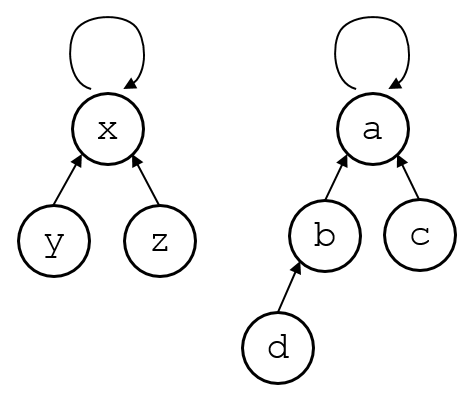
\includegraphics[height=0.4\textheight]{figures/disjoint_set}
\end{center}
\end{frame}

\begin{frame}[fragile]{Implementation Idea}
\BIT
\item \verb.Find(x).: follow the links from \verb,x, until a node points itself
\BIT
\item This can take $O(n)$ time but we will make it faster
\EIT
\vfill
\item \verb.Union(x, y).: run \verb,Find(x), and \verb,Find(y), to find corresponding root nodes and direct one to the other
\EIT
\end{frame}

\begin{frame}[fragile]{Implementation}
\BIT
\item We will assume that the links are stored in \verb.L[].
\EIT
\vfill
\begin{Verbatim}[xleftmargin=25pt]
int Find(int x) {
    while(x != L[x]) x = L[x];
    return x;
}
void Union(int x, int y) {
    L[Find(x)] = Find(y);
}
\end{Verbatim}
\end{frame}

\begin{frame}[fragile]{Path Compression}
\BIT
\item In a bad case, the trees can become too deep
\BIT
\item ... which slows down future operations
\EIT
\item Path compression makes the trees shallower every time \verb,Find(), is called
\item We don't care how a tree looks like as long as the root stays the same
\BIT
\item After \verb,Find(x), returns the root, backtrack to \verb,x, and reroute all the links to the root
\EIT
\EIT
\end{frame}

\begin{frame}[fragile]{Path Compression Implementations}
\begin{Verbatim}[xleftmargin=25pt]
int Find(int x) {
    if(x == L[x]) return x;
    int root = Find(L[x]);
    L[x] = root;
    return root;
}

int Find(int x) {
    return x == L[x] ? x : L[x] = Find(L[x]);
}
\end{Verbatim}
\end{frame}


\section{Binary Search Tree (BST)}

\begin{frame}[fragile]{Binary Search Tree (BST)}
\BIT
\item A binary tree with the following property: for each node 𝑣,
\BIT
\item value of $v \ge $ values in $v$'s left subtree
\item value of $v \le $ dvalues in $v$'s right subtree
\EIT
\EIT
\begin{center}
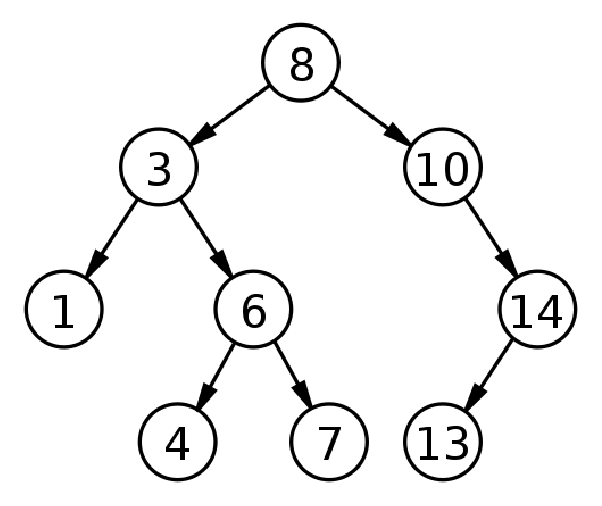
\includegraphics[height=0.4\textheight]{figures/bst}

Figure from Wikipedia
\end{center}
\end{frame}

\begin{frame}[fragile]{What BSTs can do}
\BIT
\item Supports three operations
\BIT
\item \verb,Insert(x),: inserts a node with value \verb,x,
\item \verb,Delete(x),: deletes a node with value \verb,x,, if there is any
\item \verb,Find(x),: returns the node with value \verb,x,, if there is any
\EIT
\item Many extensions are possible
\BIT
\item \verb,Count(x),: counts the number of nodes with value less than or equal to \verb,x,
\item \verb,GetNext(x),: returns the smallest node with value $\ge$ \verb,x,
\EIT
\EIT
\end{frame}

\begin{frame}[fragile]{BSTs in Programming Contests}
\BIT
\item Simple implementation cannot guarantee efficiency
\BIT
\item In worst case, tree height becomes $n$ (which makes BST useless)
\item Guaranteeing $O(\log n)$ running time per operation requires balancing of the tree (hard to implement)
\item We will skip the implementation details
\EIT
\item Use the standard library implementations
\BIT
\item \verb,set,, \verb,map, (C++)
\item \verb,TreeSet,, \verb,TreeMap, (Java)
\EIT
\EIT
\end{frame}

\section{Fenwick Tree}

\begin{frame}[fragile]{Fenwick Tree}
\BIT
\item A variant of segment trees
\item Supports very useful interval operations
\BIT
\item \verb.Set(k, x).: sets the value of \verb.k.th item equal to \verb.x.
\item \verb.Sum(k).: computes the sum of items $1, \ldots, \mathtt{k}$ (prefix sum)
\BIT
\item Note: sum of items $\mathtt{i}, \ldots, \mathtt{j} = \mathtt{Sum(j)} - \mathtt{Sum(i - 1)}$
\EIT
\EIT
\item Both operations can be done in $O(\log n)$ time using $O(n)$ space
\EIT
\end{frame}

\begin{frame}[fragile]{Fenwick Tree Structure}
\BIT
\item Full binary tree with at least $n$ leaf nodes
\BIT
\item We will use $n=8$ for our example
\EIT
\item $k$th leaf node stores the value of item $k$
\item Each internal node stores the sum of values of its children
\BIT
\item \eg, Red node stores \verb.item[5]. $+$ \verb.item[6].
\EIT
\EIT
\begin{center}
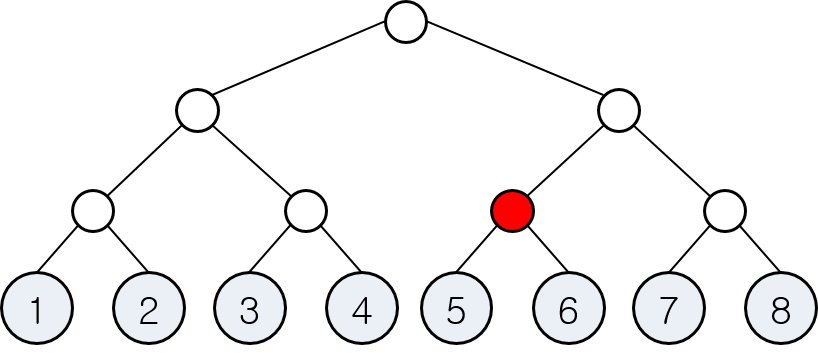
\includegraphics[height=0.4\textheight]{figures/fenwick}
\end{center}
\end{frame}

\begin{frame}{Summing Consecutive Values}
\BIT
\item Main idea: choose the minimal set of nodes whose sum gives the desired value
\item We will see that
\BIT
\item at most 1 node is chosen at each level so that the total number of nodes we look at is $\log_2 n$
\item and this can be done in $O(\log n)$ time
\EIT
\vfill
\item Let's start with some examples
\EIT
\end{frame}

\begin{frame}[fragile]{Summing: Example 1}
\BIT
\item $\mathtt{Sum(7)} = $ sum of the values of gold-colored nodes
\EIT
\begin{center}
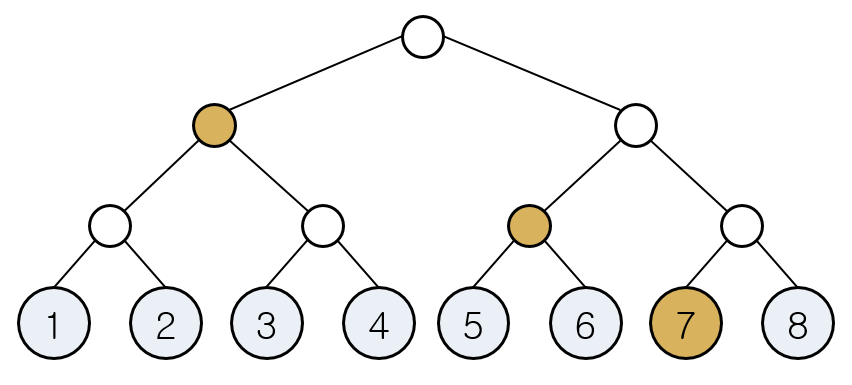
\includegraphics[height=0.4\textheight]{figures/fenwick_sum1}
\end{center}
\end{frame}

\begin{frame}[fragile]{Summing: Example 2}
\BIT
\item \verb,Sum(8),
\EIT
\begin{center}
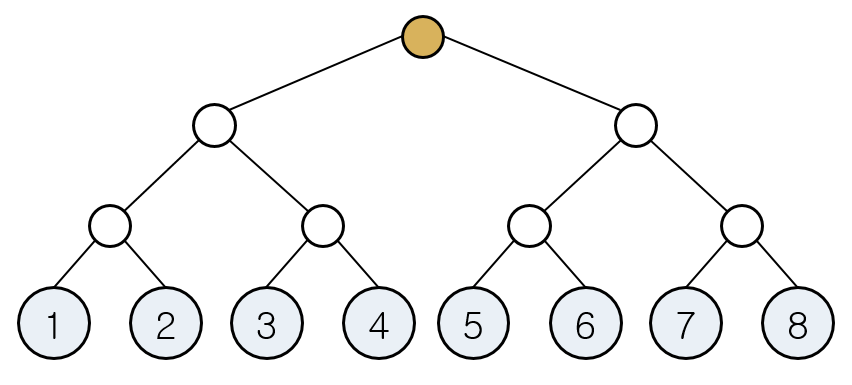
\includegraphics[height=0.4\textheight]{figures/fenwick_sum2}
\end{center}
\end{frame}

\begin{frame}[fragile]{Summing: Example 3}
\BIT
\item \verb,Sum(6),
\EIT
\begin{center}
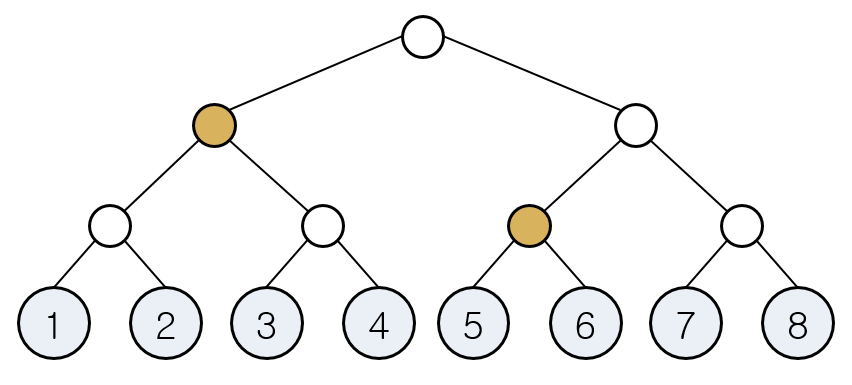
\includegraphics[height=0.4\textheight]{figures/fenwick_sum3}
\end{center}
\end{frame}

\begin{frame}[fragile]{Summing: Example 4}
\BIT
\item \verb,Sum(3),
\EIT
\begin{center}
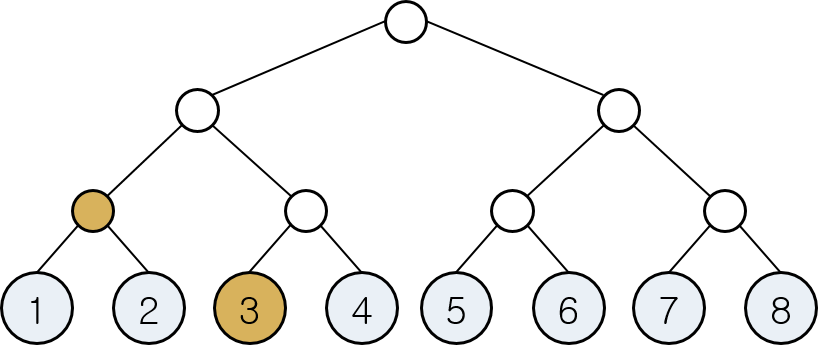
\includegraphics[height=0.4\textheight]{figures/fenwick_sum4}
\end{center}
\end{frame}

\begin{frame}[fragile]{Computing Prefix Sums}
\BIT
\item Say we want to compute \verb,Sum(k),
\item Maintain a pointer \verb,P, which initially points at leaf \verb,k,
\item Climb the tree using the following procedure:
\BIT
\item If \verb,P, is pointing to a left child of some node:
\BIT
\item Add the value of \verb,P,
\item Set \verb,P, to the parent node of \verb,P,'s left neighbor
\item If \verb,P, has no left neighbor, terminate
\EIT
\item Otherwise:
\BIT
\item Set \verb,P, to the parent node of \verb,P,
\EIT
\EIT
\item Use an array to implement (review the heap section)
\EIT
\end{frame}

\begin{frame}[fragile]{Updating a Value}
\BIT
\item Say we want to do \verb.Set(k, x). (set the value of leaf \verb,k, as \verb,x,)
\item This part is a lot easier
\item Only the values of leaf \verb,k, and its ancestors change
\EIT
\begin{enumerate}
\item Start at leaf \verb,k,, change its value to \verb,x,
\item Go to its parent, and recompute its value
\item Repeat 2 until the root
\end{enumerate}
\end{frame}

\begin{frame}[fragile]{Extension}
\BIT
\item Make the \verb,Sum(), function work for any interval
\BIT
\item ... not just ones that start from item 1
\EIT
\vfill
\item Can support more operations with the new \verb,Sum(), function
\BIT
\item \verb.Min(i, j).: Minimum element among items $\mathtt{i}, \ldots, \mathtt{j}$
\item \verb.Max(i, j).: Maximum element among items $\mathtt{i}, \ldots, \mathtt{j}$
\EIT
\EIT
\end{frame}


\section{Lowest Common Ancestor (LCA)}

\begin{frame}{Lowest Common Ancestor (LCA)}
\BIT
\item Input: a rooted tree and a bunch of node pairs
\item Output: lowest (deepest) common ancestors of the given pairs of nodes
\vfill
\item Goal: preprocessing the tree in $O(n \log n)$ time in order to answer each LCA query in $O(\log n)$ time
\EIT
\end{frame}

\begin{frame}[fragile]{Preprocessing}
\BIT
\item Each node stores its depth, as well as the links to every $2^k$th ancestor
\BIT
\item $O(\log n)$ additional storage per node
\item We will use \verb,Anc[x][k], to denote the $2^k$th ancestor of node \verb,x,
\EIT
\vfill
\item Computing \verb.Anc[x][k].:
\BIT
\item \verb.Anc[x][0] = x.'s parent
\item \verb.Anc[x][k] = Anc[ Anc[x][k-1] ][ k-1 ].
\EIT
\EIT
\end{frame}

\begin{frame}[fragile]{Answering a Query}
\BIT
\item Given two node indices \verb,x, and \verb,y,
\BIT
\item Without loss of generality, assume $\mathtt{depth(x)} \le \mathtt{depth(y)}$
\EIT
\item Maintain two pointers p and q, initially pointing at \verb,x, and \verb,y,
\item If $\mathtt{depth(p)} < \mathtt{depth(q)}$, bring \verb,q, to the same depth as \verb,p,
\BIT
\item using \verb,Anc, that we computed before
\EIT
\item Now we will assume that $\mathtt{depth(p)} = \mathtt{depth(q)}$
\EIT
\end{frame}

\begin{frame}[fragile]{Answering a Query}
\BIT
\item If \verb,p, and \verb,q, are the same, return \verb,p,
\item Otherwise, initialize \verb,k, as $\lceil \log_2 n \rceil$ and repeat:
\BIT
\item If \verb,k, is 0, return \verb,p,'s parent node
\item If \verb,Anc[p][k], is undefined, or if \verb,Anc[p][k], and \verb,Anc[q][k], point to the same node:
\BIT
\item Decrease \verb,k, by 1
\EIT
\item Otherwise:
\BIT
\item Set \verb,p = Anc[p][k], and \verb,q = Anc[q][k], to bring \verb,p, and \verb,q, up by $2^k$ levels
\EIT
\EIT
\EIT
\end{frame}

\begin{frame}[fragile]{Conclusion}
\BIT
\item We covered LOTS of stuff today
\BIT
\item Try many small examples with pencil and paper to completely internalize the material
\item Review and solve relevant problems
\EIT
\vfill
\item Discussion and collaboration are strongly recommended!
\EIT
\end{frame}

\end{document}
